\chapter{Proposed Framework}
\label{ch:Framework}

In the \autoref{ch:FeatureExtraction} the features extraction process has been described. Before aproaching the problem of performing \gls{nd} in \gls{glo:edge}, let's build a framework in \texttt{python} that runs on a \gls{pc} that is \emph{configurable}, \emph{modular}, \emph{expandable} and \emph{general purpose}. This framework will be used to test the features extraction process, and to test the \gls{ml} algorithms before selecting one of them to be implemented \gls{glo:edge} framework, that will be harder to configure.

A real case application would probably have several signals of several phisical quantities, so a general approach that can manage different types of features, and extract from each of them the most relevant information, is needed.

The proposed framework is tought to be set up on any type and combination of sensors. The framework is tought to manage data that are correlated to a specific fault. For example, think about a \gls{cnc} machines like the one in \autoref{fig:cnc}. It has five axis, so a solution would be to instance the framework five time, one for each axis, linked to vibration sensors, temperature sensor etc. of the considered axis. This would allow to pinpoint the fault to a specific axis. Another concern is, what if the single axis are seeing normal condition, but the machine as a whole is not? This may happpen if the tool has a problem: the vibration registered in the spindle are normal in general, but are not normal \emph{related} to the feedrate that another axis is imposig. To address this scenario, other instances of the framework can be set up, that also receive the speeds from the machine controlle and the feedrate from the \gls{cnc} program as well as data from the sensors used in the other instances. This would allow to detect a more complex fault, that is not characteristic of any part of the machine, but of the machine as a whole. The former kind of instances would allow to detect specific faults, giving also an idea of what the fault is, the latter would allow to detect complex faults, but would not give a precise idea of what the fault is. The framework is tought to be able to manage both of these scenarios, and to be able to manage them together.

\begin{figure}
  \centering
  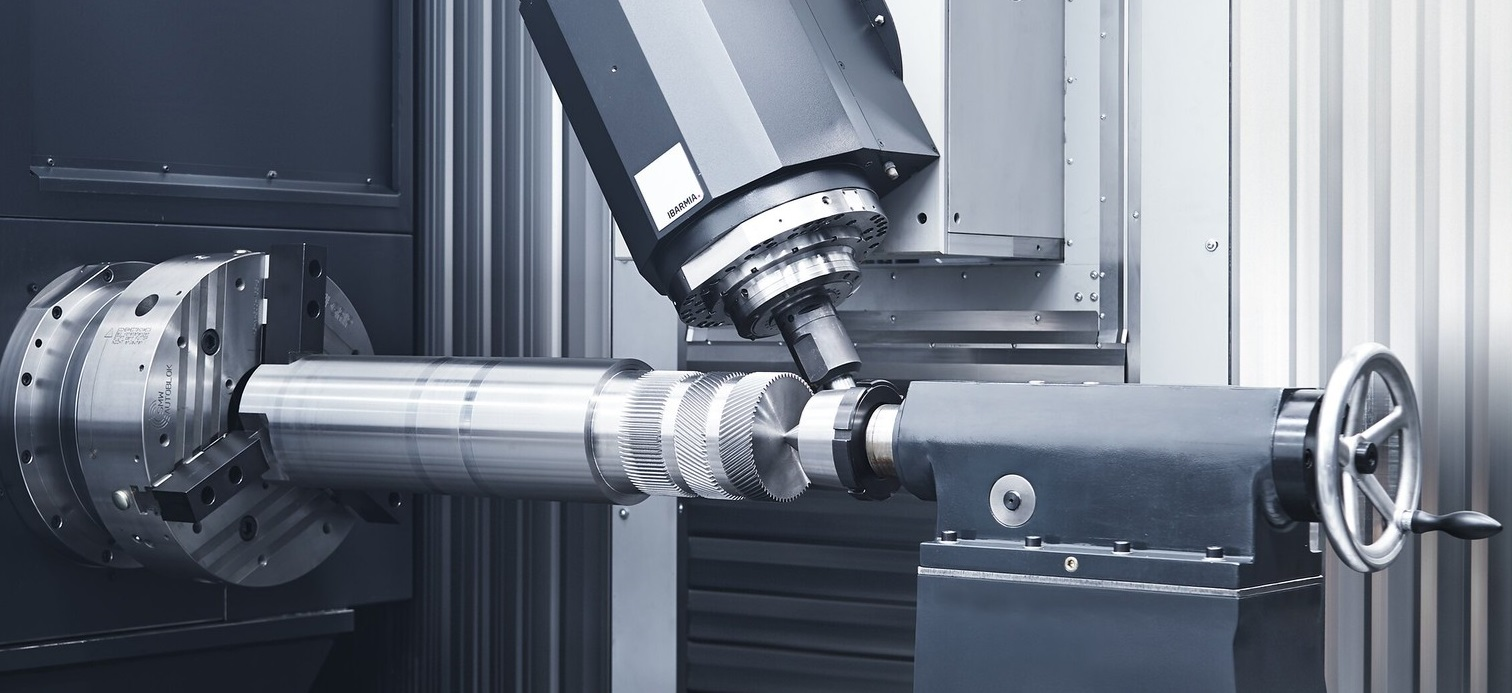
\includegraphics[width=.7\textwidth]{images/Framework/millmachine.jpg}
  \caption{A 5-axis \gls{cnc} milling machine. \cite{FagorAutomation}}
  \label{fig:cnc}
\end{figure}

\section{Commissioning}
To adapt the framework to a pecific machine, the \gls{glo:commissioning} of the \gls{ml} system would have to be done in steps. Starting from the data acquisition and ending with the predictions of \gls{glo:rul} and model updates, the steps are described in this section.

\subsection{Data acquisition}

The firts phase of the commissioning procedure is to set up the data acquisition. This has to be done when the machine is new or, at least, someone guarantees that the machine is in a healthy condition.

This include the decision of which sensors to use, the sampling frequency, the data acquisition system and which features are needed to be extracted from each the sensors data. At this point, if more than one instance of the framework is needed, the sets of sensors and features to be used in each instance are defined. For example, in a shaft with two bearings, each with two accelerometers, the first instance of the framework would be linked to the first bearing, and would use the data from the two accelerometers to extract the features that are needed to detect the fault in the first bearing. The second instance of the framework would be linked to the second bearing, and would use the data from the other two accelerometers to extract the features that are needed to detect the fault in the second bearing. Optionally, a third instance of the framework would use the data from all the four accelerometers to detect a generic fault in the shaft.
Those decisions influence the structure of the database, that is described in \autoref{sec:Database}. 

\section{Database}
\label{sec:Database}
As first thing, let's address the problem of storing the data in an efficient and effective way. Instead of relying on python data structures, let's use a database. 
MongoDB is a widely-used, open-source \gls{glo:nosql} database that is designed to handle unstructured or semi-structured data. It utilizes a document-oriented data model, storing data in flexible, \gls{json}-like \gls{bson} format. MongoDB is suitable for implementation in a \gls{nd} framework due to its scalability, flexibility, and real-time data processing capabilities. In novelty detection, the system often deals with diverse and dynamic data sources, making MongoDB's \quoted{unstructureness} advantageous for handling varying data formats and evolving data requirements. It has the ability to handle large volumes of data and support scaling allows for efficient storage and retrieval of information in real-time, crucial for real-time applications. Moreover, MongoDB has a rich query language and secondary indexes that allow for fast and efficient querying of data and a library for \texttt{python} that makes it easy to use.
The \gls{json} format is also human-readable, which makes it easy to understand the data stored in the database, and \quoted{mongoDB Compass} is a graphical user interface that allows to easily explore the database.

\subsection{Collections}
\begin{longtblr}[
    caption = {Collections contained in the mongoDB database},
    label = {tab:MongoDB_collections},
  ]{
    hline{1,11} = {-}{0.08em},
    hline{2} = {-}{},
  }
  \textbf{Collection} & \textbf{Content}\\
  raw & time-series and information about them\\
  unconsumed & snapshots to be evaluated\\
  quarantined & {snapshots detected as novelty waiting to be declared\\healthy, faulty or be discarded}\\
  healthy & snapshots declared as normal behaviour\\
  healthy train & {training dataset (scaled, processed, packet)\\for the \gls{nd} \gls{uml} model}\\
  faulty & snapshots declared as faulty behaviour\\
  faulty train & {training dataset (scaled, processed, packet)\\for the \gls{nd} \gls{uml} model}\\
  models & {models trained on healthy and faulty data the metrics \\and predictions to be shown}\\
  backup & timeseries, features, models, etc.
  \end{longtblr}

MongoDB structure is based on collections, that are groups of (\gls{json}) documents. A document is a set of key-value pairs. Documents have dynamic schema, which means that documents in the same collection do not need to have the same set of fields or structure, and common fields in a collection's documents may hold different types of data. To store the data needed by the framework the collections reported in \autoref{tab:MongoDB_collections} are used.

\paragraph{Raw}
Thinking about the data flow, the first interface between the hardware and the software would be the sensor readings. Every sensor should have a name and be sampled at a constant frequency (or, at least, the sensors that provide data for frequency-domain feature extraction should have a constant sampling frequency). This data is stored in the {raw} collection, with the following \gls{json} structure:
\begin{lstlisting}[language=json,firstnumber=1]
    {
        "_id": {
          "$oid": "xx...xxx"
        },
        "timestamp": {
          "$date": "YYYY-MM-DDThh:mm:ss.SSSZ"
        },
        "Sensor 1": {
          "sampFreq": 123456,
          "timeSerie": [
            123.456,
            . . . ,
            123.456
          ]
        },
        ...
        "Sensor n": {
          "sampFreq": 123456,
          "timeSerie": [
            -123.456,
            . . . ,
            123.456
          ]
        }
      }
\end{lstlisting}
where \texttt{\_id} is the unique identifier of the document, \texttt{timestamp} is the time at which the data was acquired, in \gls{iso} format, and \texttt{Sensor 1} to \texttt{Sensor n} are the sensors names. Each sensor has a \texttt{sampFreq} field that contains the sampling frequency of that particular sensor, and a \texttt{timeSerie} field that contains the data acquired by the sensor, as a list. The \texttt{timeSerie} field is a list of floating point numbers, that can be of any length. Note that the sampling frequencies of different sensors can be different, for example if a timestamp contains $1\si{\s}$ worth of data, a vibration sensor would be linked to an array with several thousands of samples, while a temperature sensor would be linked to only one sample.

\paragraph{Unconsumed}
Once defined the structure that the timeseries will have in the database, let's define the structure of the snapshots. The features extracted from the timeseries are stored in the {unconsumed} collection, with the following \gls{json} structure:

\begin{lstlisting}[language=json,firstnumber=1]
    {
        "_id": {
          "$oid": "xxx....xxx"
        },
        "timestamp": {
          "$date": "YYY-MM-DDThh:mm:ss.SSSZ"
        },
        "Sensor 1": {
          "mean": 123.456,
          "rms": 123.456,
          "peak2peak": 123.456,
          "std": 123.456,
          "skewness": 123.456,
          "kurtosis": 123.456,
          "wavelet coef aaaaaa": 123.456,
          "wavelet coef aaaaad": 123.456,
          ...,
          "wavelet coef dddddd": 123.456
        },
        "Sensor 2": {
          "mean": 123.456,
          "kurtosis": 1.099722740047154
        },
        ...,
        "Sensor n": {
          "mean": 123.456,
          ...
        }
        "novelty evaluated": true/false
      }
\end{lstlisting}

Notice that different sensors can have different features. The \quoted{novelty evaluated} field is a boolean that is set to \texttt{false} when the snapshot is created, and is set to \texttt{true} when the \gls{nd} algorithm evaluates the snapshot. This field is used to avoid evaluating the same snapshot multiple times, while leaving it in the collection untill also the \gls{fd} algorithm will be performed. At this point the snapshot will be moved either to the backup collection, discarded or to the quarantine collection if either the \gls{nd} or the \gls{fd} flag it.

\paragraph{Quarantined}
The \quoted{quarantined} collection is used to store the snapshots that were flagged as \quoted{novelty} by the \gls{nd} algorithm or as \quoted{faulty} by the \gls{fd} algorithm (or were flagged by both of them). The structure is the same as the \quoted{unconsumed} collection, but the \quoted{novelty evaluated} field is not present since, at this point, the snapshots are guaranteed to have been evaluated. The snapshots in this collection are waiting to be declared as \quoted{healthy} or \quoted{faulty} by the user, or to be discarded.

\paragraph{Healthy}
The idea behind the \quoted{healthy} collection is to store the snapshots that are aquired during the first work-phase of the framework, before training, or the snapshots that were in the \quoted{quarantine} collection and were declared as healthy by the user. The documents in this collection have the same structure as the documents in the \quoted{quarantined} collection.

\paragraph{Healthy train}
In this collection the healthy snapshots are packed together in different document, each of htem useful in a different phase of the training process. 

{The first document hase the \texttt{id} \texttt{training\_set}, that contains all the \texttt{N} training snapshots, each of them with \texttt{n} sensors signals, characterized by \texttt{F} features. For ease of accessibility, every bottom-nested field is a list of \texttt{N} elements. The structure is the following:}

\begin{lstlisting}[language=json,firstnumber=1]
{
  "_id": "training set",
  "timestamp": [
    {
      "$date": "YYYY-MM-DDThh:mm:ss.SSSZ" 	# timestamp 1
    },  
	...,
    {   
      "$date": "YYYY-MM-DDThh:mm:ss.SSSZ" 	# timestamp N
    }
  ],
  "Sensor 1": {
    "Feature 1": [
      123.456,								# value 1
      ...,
      123.456								# value N
    ],
	...,
	"Feature F": [
      123.456,								# value 1
      ...,
      123.456								# value N
    ]},
	...
  "Sensor n": {
    "Feature 1": [
      123.456,								# value 1
      ...,
      123.456								# value N
    ],
	...,
	"Feature F": [
      123.456,								# value 1
      ...,
      123.456								# value N
    ]}
}
\end{lstlisting}

\paragraph{Faulty}
This collection serve the same exact purpose as the \quoted{healthy} collection, but for the faulty snapshots. Faulty snapshots are not discarded because they can be used to train the \gls{fd} \gls{uml} algorithm.

\paragraph{Faulty train}

\paragraph{Models}


\paragraph{Backup}

\begin{figure}
    \centering
    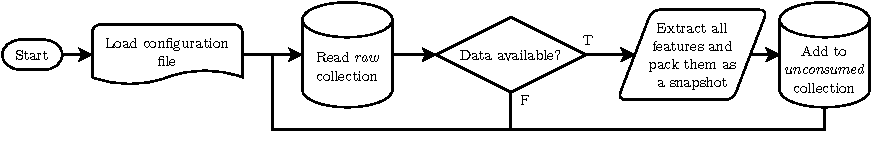
\includegraphics[width=\textwidth]{images/Framework/FA_flowchart.pdf}
    \caption{Feature Agent flowchart}
    \label{fig:FA_flowchart}
\end{figure}

\begin{figure}
    \centering
    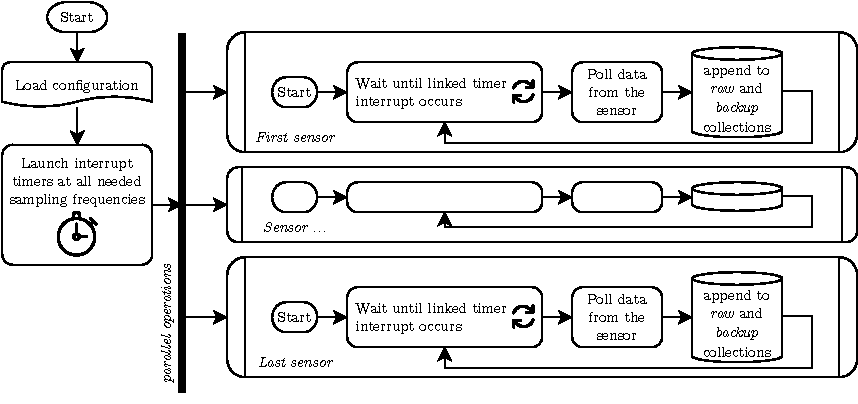
\includegraphics[scale=1]{images/Framework/Field_Agent_flowchart.pdf}
    \caption{Field Agent flowchart}
    \label{fig:Field_Agent_flowchart}
\end{figure}

\begin{figure}
    \centering
    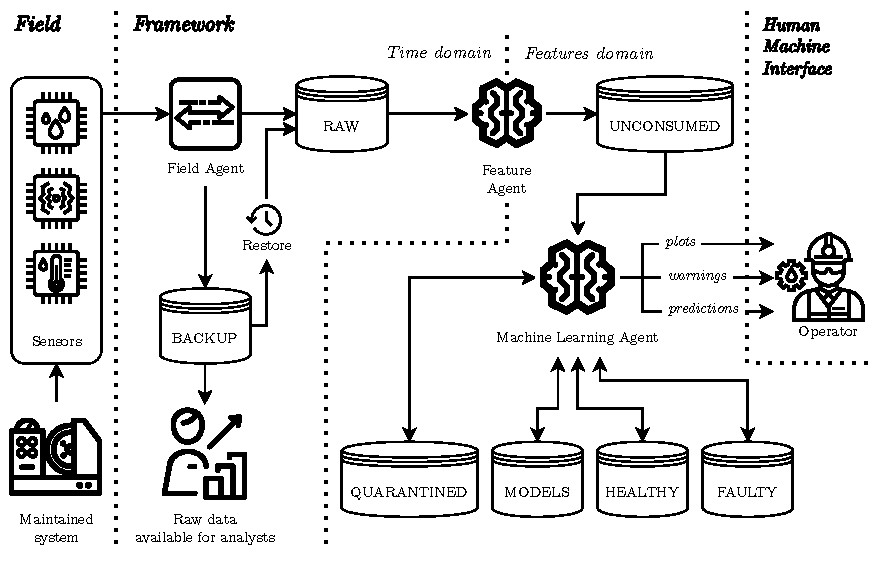
\includegraphics[width=\textwidth]{images/Framework/Framework_structure.pdf}
    \caption{Framework locical structure}
    \label{fig:Framework_structure}
\end{figure}

\begin{figure}
    \centering
    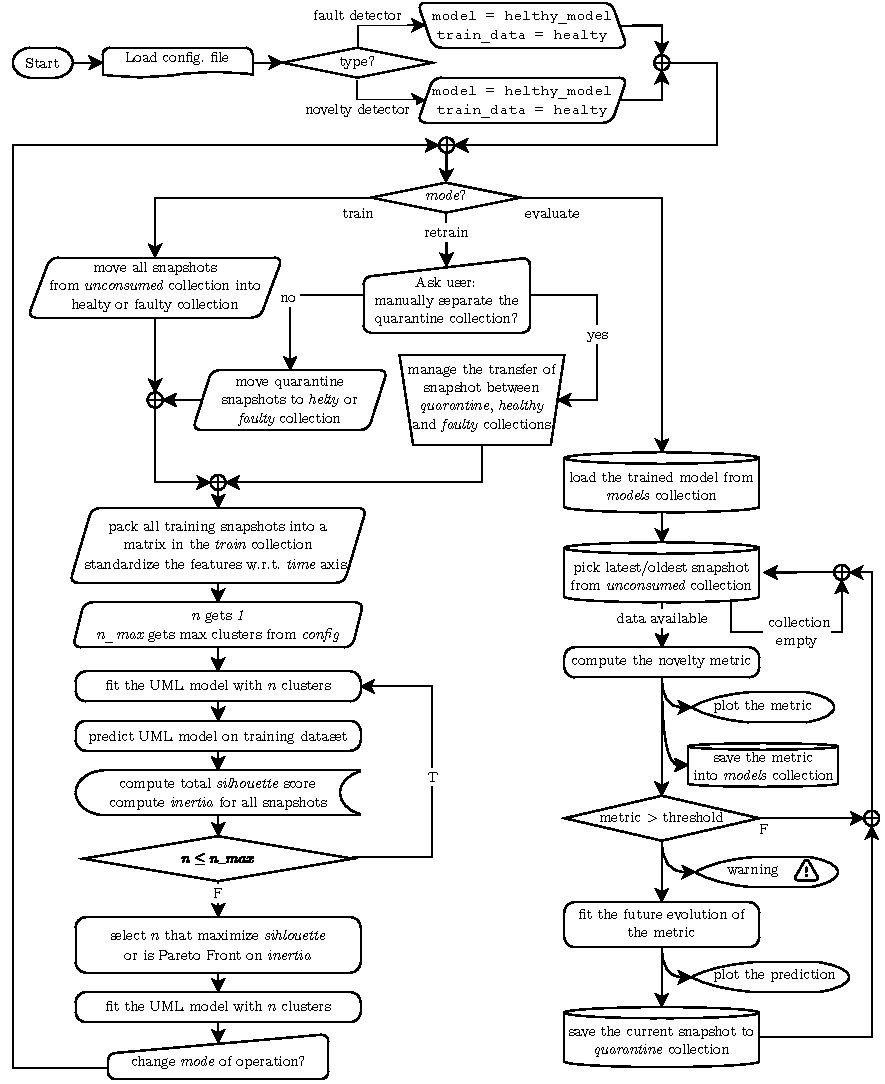
\includegraphics[width=\textwidth]{images/Framework/MLA.pdf}
    \caption{Machine Learning Agent flowchart. When it is instanced for \gls{nd}, the \gls{mla} uses the healthy collection as training dataset, when it is instanced for \gls{fd} it uses the faulty collection.}
    \label{fig:MLA_structure}
\end{figure}


